% -------------Welcome to your first LaTeX document with R code!
% The following is a Bare bones Sweave (R + LaTex) document for creating APA style papers

% Important
%   1) Make sure you've installed the latest version of the knitr package with install.packages('knitr')
%   2) Set RStudio preferences to Sweave with knitr: RStudio -- Preferences -- Sweave -- Weave Rnw files with knitr


\documentclass[a4paper,man,natbib,floatsintext]{apa6}\usepackage[]{graphicx}\usepackage[]{color}
%% maxwidth is the original width if it is less than linewidth
%% otherwise use linewidth (to make sure the graphics do not exceed the margin)
\makeatletter
\def\maxwidth{ %
  \ifdim\Gin@nat@width>\linewidth
    \linewidth
  \else
    \Gin@nat@width
  \fi
}
\makeatother

\definecolor{fgcolor}{rgb}{0.345, 0.345, 0.345}
\newcommand{\hlnum}[1]{\textcolor[rgb]{0.686,0.059,0.569}{#1}}%
\newcommand{\hlstr}[1]{\textcolor[rgb]{0.192,0.494,0.8}{#1}}%
\newcommand{\hlcom}[1]{\textcolor[rgb]{0.678,0.584,0.686}{\textit{#1}}}%
\newcommand{\hlopt}[1]{\textcolor[rgb]{0,0,0}{#1}}%
\newcommand{\hlstd}[1]{\textcolor[rgb]{0.345,0.345,0.345}{#1}}%
\newcommand{\hlkwa}[1]{\textcolor[rgb]{0.161,0.373,0.58}{\textbf{#1}}}%
\newcommand{\hlkwb}[1]{\textcolor[rgb]{0.69,0.353,0.396}{#1}}%
\newcommand{\hlkwc}[1]{\textcolor[rgb]{0.333,0.667,0.333}{#1}}%
\newcommand{\hlkwd}[1]{\textcolor[rgb]{0.737,0.353,0.396}{\textbf{#1}}}%
\let\hlipl\hlkwb

\usepackage{framed}
\makeatletter
\newenvironment{kframe}{%
 \def\at@end@of@kframe{}%
 \ifinner\ifhmode%
  \def\at@end@of@kframe{\end{minipage}}%
  \begin{minipage}{\columnwidth}%
 \fi\fi%
 \def\FrameCommand##1{\hskip\@totalleftmargin \hskip-\fboxsep
 \colorbox{shadecolor}{##1}\hskip-\fboxsep
     % There is no \\@totalrightmargin, so:
     \hskip-\linewidth \hskip-\@totalleftmargin \hskip\columnwidth}%
 \MakeFramed {\advance\hsize-\width
   \@totalleftmargin\z@ \linewidth\hsize
   \@setminipage}}%
 {\par\unskip\endMakeFramed%
 \at@end@of@kframe}
\makeatother

\definecolor{shadecolor}{rgb}{.97, .97, .97}
\definecolor{messagecolor}{rgb}{0, 0, 0}
\definecolor{warningcolor}{rgb}{1, 0, 1}
\definecolor{errorcolor}{rgb}{1, 0, 0}
\newenvironment{knitrout}{}{} % an empty environment to be redefined in TeX

\usepackage{alltt}
% To see your document in publication format, change "doc" to "pub"
% To put the figures at the end of the document, remove the floatsintext argument above.

\usepackage{filecontents}

% Now we'll define the titles of the paper, and the authors of our manuscript
\title{Bare-bones Sweave Document}
\shorttitle{sweave}
\author{Nathaniel D. Phillips}
\affiliation{University of Basel}

% Now, we write our abstract in the abstract command
\abstract{This is an example APA style paper written in Sweave -- a combination of LaTeX and R code.}

% Here are the keywords to our article
\keywords{sweave, r, latex, apa}

% The begin{document} and maketitle commands start the actual document and creates the title page
\IfFileExists{upquote.sty}{\usepackage{upquote}}{}
\begin{document}
\SweaveOpts{concordance=TRUE}
%\SweaveOpts{concordance=TRUE}
\maketitle





\section{Introduction}

In \cite{bargh1996automaticity} published a provocative paper that tested whether submliminal primes affect unconscious behavior. In Experiment 2a of their paper, they found that people given primes related to elderly stereotypes subsequently walked slower than those given neutral primes.

In this paper I will try to replicate and extend results (with \emph{fictional} data) across two studies. In study 1, I will attempt to replicate their effect of primes on unconscious behavior (i.e.; walking speed). In study 2, I will extend their paradigm to test if unconscious primes affect deliberate decision making behavior (i.e.; deciding whether or not to make a monetary donation).

I have two hypotheses:

\subsection{Hypotheses}

\begin{enumerate}

  \item[H1] Participants given an elderly prime will walk slower (automatic behavior) than those given a neutral prime (Study 1).
  \item[H2] Participants given an elderly prime will be more likely to donate to a charity (deliberate decision making) for the elderly compared to those given a neutral prime (Study 2).

\end{enumerate}

\section{Study 1}

In study 1, I tested Hypothesis 1 in a direct replication of Experiment 2a of \cite{bargh1996automaticity}.




\subsection{Method}

\subsubsection{Participants}

100 students (53\% female) participated in exchange for course credit. The mean age was 22.21

\subsubsection{Materials}

The priming manipulation took the form of a scrambled-sentence task presented to participants as a test of language proficiency. We constructed two versions of the scrambled sentence task: one elderly prime version, which contained words related to the elderly stereotype, and another, neutral version. For the elderly prime version, the critical stimuli were worried, Florida, old, lonely, grey, selfishly, careful, sentimental, wise, stubborn, courteous, bingo, withdraw,forgetfuL retired, wrinkle, rigid, traditional bitter, obedient, conservative, knits, dependent, ancient, helpless, gullible, cautious, and alone. These prime words were obtained from previous research that examined the components of the elderly stereotype \citep{brewer1981perceptions, harris1976myth, mctavish1971perceptions, perdue1990evidence}. In the neutral version, the elderly prime words were replaced with the words unrelated to the elderly stereotype (e.g., thirsty, clean, private).


\subsubsection{Procedure}

Our (again, fictional) study folled the exact same procedure as \cite{bargh1996automaticity}. What follows is a \emph{verbatim} description of their procedure from their Experiment 2a.

Participants took part in the experiment one at a time. The participant was informed that the purpose of the study was to investigate language proficiency and that he or she was to complete a scrambled-sentence task. The task consisted of 30 sets of fiveword com- binations. The participant was instructed to write down a grammati- cally correct sentence using only four of the five words given. Partici- pants were also informed that the task was self-paced. After giving the instructions, the experimenter left the room so that the participant could complete the task in privacy.

After the participant completed the task and notified the experi- menter, the experimenter re-entered the lab room and partially de- briefed the participant. He or she was informed that the experiment was concerned with how individuals use words in various, flexible ways. Waiting until the participant had gathered all of his or her belongings, the experimenter told the participant that the elevator was down the hall and thanked him or her for participating.

Using a hidden stopwatch, a confederate of the experimenter, who was sitting in a chair apparently waiting to talk to a professor in a nearby office, recorded the amount of time in seconds that the participant spent walking a length of the corridor starting from the doorway of the experimental room and ending at a broad strip of silver carpet tape on the floor 9.75 m away.

Afterward, the experimenter caught up with the participant near the elevator and gave the complete debriefing, explaining the experimental hypotheses verbally as well as giving the participant an accompanying written version. Participants were also informally asked (prior to this final debriefing) whether they thought the scrambled-sentence task might have affected them in any way, and if they had known that the task contained words relevant to the elderlystereotype. No participant expressed any knowledge of the relevance of the words in the scrambled-sentence task to the elderly stereotype. Furthermore, no participant believed that the words had an impact on his or her behavior.

\subsection{Results}




A boxplot of the walking times by condition are presented in Figure~\ref{fig:s1times}. The mean walking time of those in the elderly prime condition was 10.87. In the neutral prime condition, the mean time was 9.8.

\begin{figure}
\begin{knitrout}
\definecolor{shadecolor}{rgb}{0.969, 0.969, 0.969}\color{fgcolor}

{\centering 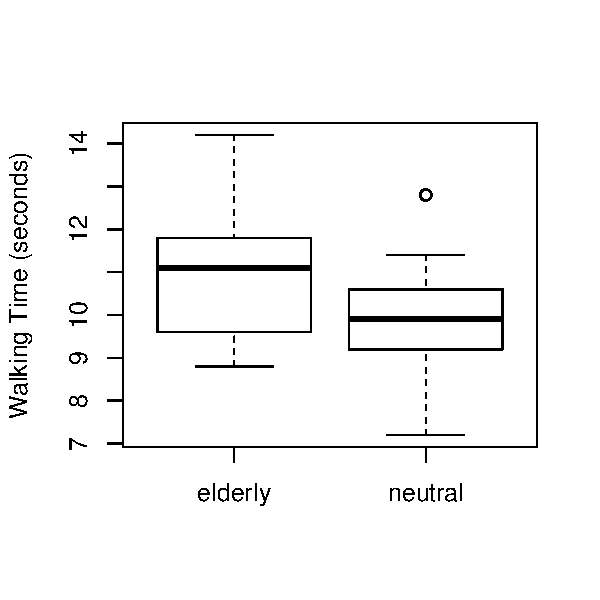
\includegraphics[width=\maxwidth]{figure/unnamed-chunk-4-1} 

}



\end{knitrout}
\caption{Distribution of walking times by priming condition in Study 1.}
\label{fig:s1times}
\end{figure}




To test the effects of the prime on walking speed, I conducted a two-sample t-test. The result was significant (t(97.24) = 4.52, p < .001) and consistent with Hypothesis 1.

\subsection{Discussion}

Study 1 confirmed Hypothesis 1 and appeared to replicate the results of \cite{bargh1996automaticity}. However, it's unclear if priming would affect decision making in addition to automatic behavior (walking speed). To fill this gap, I ran study 2.

\section{Study 2}

In Study 2 I replicated Study 1 with a new dependent variable assessing people's conscious decision making process. Now, after the prime I asked people if they would be willing to donate money to a charity for the elderly.

\subsection{Method}


\subsubsection{Participants}

150 students (49\% female) participated in exchange for course credit. The mean age was 21.9.

\subsubsection{Procedure}

The procedure for Study 2 was identical to that of Study 1. The only differene was that after participants walked down the hall, I asked them if they would be willing to donate \$10 to a charity in support of the elderly.

\subsection{Results}

 A barplot of the donation rates by condition are presented in Figure~\ref{fig:s2donation}.





\begin{figure}
\begin{knitrout}
\definecolor{shadecolor}{rgb}{0.969, 0.969, 0.969}\color{fgcolor}

{\centering 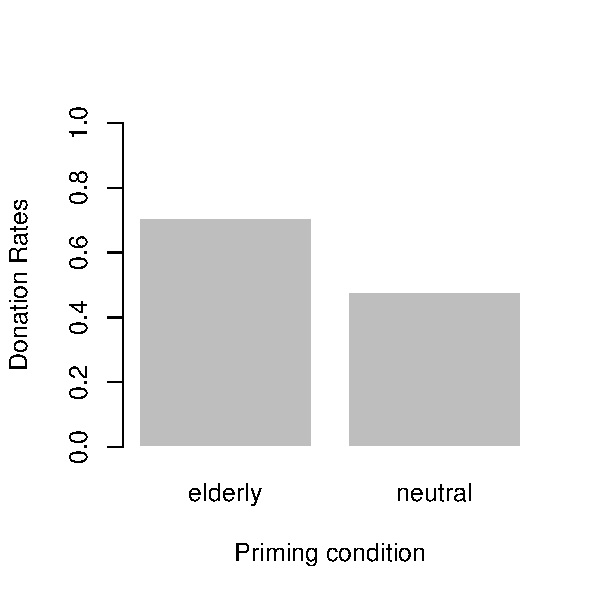
\includegraphics[width=\maxwidth]{figure/unnamed-chunk-7-1} 

}



\end{knitrout}
\caption{Donation rates by priming condition in study 2.}
\label{fig:s2donation}
\end{figure}



In the neutral priming condition 48\% participants donated to the charity. In the elderly prime condition, this proportion increased to  71\%.



A frequentist chi-square test found a significant effect of priming condition on donation rates ($X^{2}$(1) = 7.07, p < .01)


\section{General Discussion}

In two (made-up) studies, I replicated and extended the effects of unconscious priming on behavior initially reported by \cite{bargh1996automaticity}.

\section{Conclusion}

Sweave is awesome.

\begin{filecontents}{mybibliography.bib}

@article{bargh1996automaticity,
  title={Automaticity of social behavior: Direct effects of trait construct and stereotype activation on action.},
  author={Bargh, John A and Chen, Mark and Burrows, Lara},
  journal={Journal of personality and social psychology},
  volume={71},
  number={2},
  pages={230},
  year={1996},
  publisher={American Psychological Association}
}

@article{morey2015package,
  title={Package 'BayesFactor'},
  author={Morey, Richard D and Rouder, Jeffrey N and Jamil, Tahira and Morey, Maintainer Richard D},
  year={2015}
}

@book{harris1976myth,
  title={The myth and reality of aging in America},
  author={Harris, Louis and National Council on the Aging},
  year={1976},
  publisher={Washington: National Council on the Aging, c1975, 1976 printing.}
}

@article{perdue1990evidence,
  title={Evidence for the automaticity of ageism},
  author={Perdue, Charles W and Gurtman, Michael B},
  journal={Journal of Experimental Social Psychology},
  volume={26},
  number={3},
  pages={199--216},
  year={1990},
  publisher={Elsevier}
}

@article{mctavish1971perceptions,
  title={Perceptions of old people: A review of research methodologies and findings.},
  author={McTavish, Donald G},
  journal={The gerontologist},
  year={1971},
  publisher={Gerontological Society of America}
}


@article{brewer1981perceptions,
  title={Perceptions of the elderly: Stereotypes as prototypes.},
  author={Brewer, Marilynn B and Dull, Valerie and Lui, Layton},
  journal={Journal of Personality and Social Psychology},
  volume={41},
  number={4},
  pages={656},
  year={1981},
  publisher={American Psychological Association}
}

@article{srull1979role,
  title={The role of category accessibility in the interpretation of information about persons: Some determinants and implications.},
  author={Srull, Thomas K and Wyer, Robert S},
  journal={Journal of Personality and Social psychology},
  volume={37},
  number={10},
  pages={1660},
  year={1979},
  publisher={American Psychological Association}
}

\end{filecontents}


\bibliography{mybibliography.bib}
\end{document}
